\subsection*{Level 1}
The part for following the model was derived by inverting each block of the DC
motor model step by step. This was then verified by using outputs from the DC
motor model as input to the inversed model. This should result in that
the input to the DC motor model is the same as the output for the
inverse model. Since this is the case, this part can be seen as
verified. \\ 
\par Values for $a_{max}$ and $v_{max}$ needed to be
obtained in order to design the trajectory planner. $v_{max}$ was read
from the velocity plot when the motor model was fed with 24 V. $a_{max}$
was calculated to a value around 650 \si{\meter\per\square\second} but
since this value saturates the voltage from the model follower,
therefore was $a_{max}$ tweaked into a value which never saturated the
voltage. These derived values can be seen in Table~\ref{tbl:table1}.
\begin{table}[H]
    \centering
    \caption{Max values for acceleration and velocity}
	\begin{tabular}{| c | c |}
        \hline
	    $a_{max}$ & 255 \\ \hline
		$v_{max}$ & 270 \\ 
		\hline
	\end{tabular}
        \label{tbl:table1}
\end{table}
The signal from the trajectory planner with Rs = 10 and Rs=100 can be seen in Figure \ref{fig:task2_pos}.

\begin{figure}[H]
	\begin{center}
	
		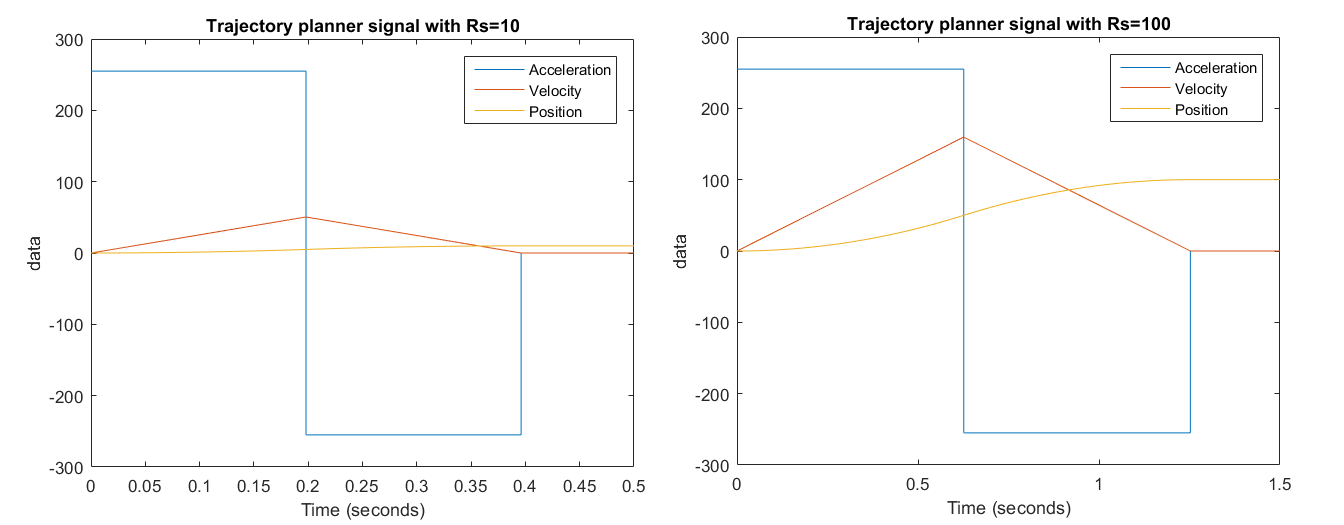
\includegraphics[width=0.90\linewidth]{task1_traj_rs10.png}
		\caption{The trajectory planner with different Rs values}
		\label{fig:task2_pos}
	\end{center}
\end{figure}
